\section{Neurophenomenology of KT}


\begin{frame}[label=ladila]{The dimensions of structured experience}
  
 \begin{center}%\includegraphics[height=1.2cm]{COPL}%
  %\hspace{2cm}
  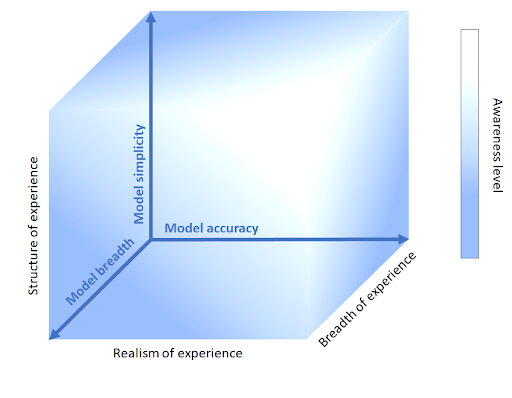
\includegraphics[height=7cm]{img/3dKT.png}
  \end{center}
  
   %Model features (simplicity, breadth, and accuracy) vs. neurophenomenology in KT. The panel displays objective model aspects, i.e., how simple/short the model/program is, how much data from input/output interfaces of the agent it tries to account for, and how well it matches data; and how these dimensions map into the level of \SEP (called awareness in the colorbar).
 
\end{frame}

